% Options for packages loaded elsewhere
\PassOptionsToPackage{unicode}{hyperref}
\PassOptionsToPackage{hyphens}{url}
\PassOptionsToPackage{dvipsnames,svgnames,x11names}{xcolor}
%
\documentclass[
  letterpaper,
  DIV=11,
  numbers=noendperiod]{scrartcl}

\usepackage{amsmath,amssymb}
\usepackage{iftex}
\ifPDFTeX
  \usepackage[T1]{fontenc}
  \usepackage[utf8]{inputenc}
  \usepackage{textcomp} % provide euro and other symbols
\else % if luatex or xetex
  \usepackage{unicode-math}
  \defaultfontfeatures{Scale=MatchLowercase}
  \defaultfontfeatures[\rmfamily]{Ligatures=TeX,Scale=1}
\fi
\usepackage{lmodern}
\ifPDFTeX\else  
    % xetex/luatex font selection
\fi
% Use upquote if available, for straight quotes in verbatim environments
\IfFileExists{upquote.sty}{\usepackage{upquote}}{}
\IfFileExists{microtype.sty}{% use microtype if available
  \usepackage[]{microtype}
  \UseMicrotypeSet[protrusion]{basicmath} % disable protrusion for tt fonts
}{}
\makeatletter
\@ifundefined{KOMAClassName}{% if non-KOMA class
  \IfFileExists{parskip.sty}{%
    \usepackage{parskip}
  }{% else
    \setlength{\parindent}{0pt}
    \setlength{\parskip}{6pt plus 2pt minus 1pt}}
}{% if KOMA class
  \KOMAoptions{parskip=half}}
\makeatother
\usepackage{xcolor}
\setlength{\emergencystretch}{3em} % prevent overfull lines
\setcounter{secnumdepth}{-\maxdimen} % remove section numbering
% Make \paragraph and \subparagraph free-standing
\ifx\paragraph\undefined\else
  \let\oldparagraph\paragraph
  \renewcommand{\paragraph}[1]{\oldparagraph{#1}\mbox{}}
\fi
\ifx\subparagraph\undefined\else
  \let\oldsubparagraph\subparagraph
  \renewcommand{\subparagraph}[1]{\oldsubparagraph{#1}\mbox{}}
\fi

\usepackage{color}
\usepackage{fancyvrb}
\newcommand{\VerbBar}{|}
\newcommand{\VERB}{\Verb[commandchars=\\\{\}]}
\DefineVerbatimEnvironment{Highlighting}{Verbatim}{commandchars=\\\{\}}
% Add ',fontsize=\small' for more characters per line
\usepackage{framed}
\definecolor{shadecolor}{RGB}{241,243,245}
\newenvironment{Shaded}{\begin{snugshade}}{\end{snugshade}}
\newcommand{\AlertTok}[1]{\textcolor[rgb]{0.68,0.00,0.00}{#1}}
\newcommand{\AnnotationTok}[1]{\textcolor[rgb]{0.37,0.37,0.37}{#1}}
\newcommand{\AttributeTok}[1]{\textcolor[rgb]{0.40,0.45,0.13}{#1}}
\newcommand{\BaseNTok}[1]{\textcolor[rgb]{0.68,0.00,0.00}{#1}}
\newcommand{\BuiltInTok}[1]{\textcolor[rgb]{0.00,0.23,0.31}{#1}}
\newcommand{\CharTok}[1]{\textcolor[rgb]{0.13,0.47,0.30}{#1}}
\newcommand{\CommentTok}[1]{\textcolor[rgb]{0.37,0.37,0.37}{#1}}
\newcommand{\CommentVarTok}[1]{\textcolor[rgb]{0.37,0.37,0.37}{\textit{#1}}}
\newcommand{\ConstantTok}[1]{\textcolor[rgb]{0.56,0.35,0.01}{#1}}
\newcommand{\ControlFlowTok}[1]{\textcolor[rgb]{0.00,0.23,0.31}{#1}}
\newcommand{\DataTypeTok}[1]{\textcolor[rgb]{0.68,0.00,0.00}{#1}}
\newcommand{\DecValTok}[1]{\textcolor[rgb]{0.68,0.00,0.00}{#1}}
\newcommand{\DocumentationTok}[1]{\textcolor[rgb]{0.37,0.37,0.37}{\textit{#1}}}
\newcommand{\ErrorTok}[1]{\textcolor[rgb]{0.68,0.00,0.00}{#1}}
\newcommand{\ExtensionTok}[1]{\textcolor[rgb]{0.00,0.23,0.31}{#1}}
\newcommand{\FloatTok}[1]{\textcolor[rgb]{0.68,0.00,0.00}{#1}}
\newcommand{\FunctionTok}[1]{\textcolor[rgb]{0.28,0.35,0.67}{#1}}
\newcommand{\ImportTok}[1]{\textcolor[rgb]{0.00,0.46,0.62}{#1}}
\newcommand{\InformationTok}[1]{\textcolor[rgb]{0.37,0.37,0.37}{#1}}
\newcommand{\KeywordTok}[1]{\textcolor[rgb]{0.00,0.23,0.31}{#1}}
\newcommand{\NormalTok}[1]{\textcolor[rgb]{0.00,0.23,0.31}{#1}}
\newcommand{\OperatorTok}[1]{\textcolor[rgb]{0.37,0.37,0.37}{#1}}
\newcommand{\OtherTok}[1]{\textcolor[rgb]{0.00,0.23,0.31}{#1}}
\newcommand{\PreprocessorTok}[1]{\textcolor[rgb]{0.68,0.00,0.00}{#1}}
\newcommand{\RegionMarkerTok}[1]{\textcolor[rgb]{0.00,0.23,0.31}{#1}}
\newcommand{\SpecialCharTok}[1]{\textcolor[rgb]{0.37,0.37,0.37}{#1}}
\newcommand{\SpecialStringTok}[1]{\textcolor[rgb]{0.13,0.47,0.30}{#1}}
\newcommand{\StringTok}[1]{\textcolor[rgb]{0.13,0.47,0.30}{#1}}
\newcommand{\VariableTok}[1]{\textcolor[rgb]{0.07,0.07,0.07}{#1}}
\newcommand{\VerbatimStringTok}[1]{\textcolor[rgb]{0.13,0.47,0.30}{#1}}
\newcommand{\WarningTok}[1]{\textcolor[rgb]{0.37,0.37,0.37}{\textit{#1}}}

\providecommand{\tightlist}{%
  \setlength{\itemsep}{0pt}\setlength{\parskip}{0pt}}\usepackage{longtable,booktabs,array}
\usepackage{calc} % for calculating minipage widths
% Correct order of tables after \paragraph or \subparagraph
\usepackage{etoolbox}
\makeatletter
\patchcmd\longtable{\par}{\if@noskipsec\mbox{}\fi\par}{}{}
\makeatother
% Allow footnotes in longtable head/foot
\IfFileExists{footnotehyper.sty}{\usepackage{footnotehyper}}{\usepackage{footnote}}
\makesavenoteenv{longtable}
\usepackage{graphicx}
\makeatletter
\def\maxwidth{\ifdim\Gin@nat@width>\linewidth\linewidth\else\Gin@nat@width\fi}
\def\maxheight{\ifdim\Gin@nat@height>\textheight\textheight\else\Gin@nat@height\fi}
\makeatother
% Scale images if necessary, so that they will not overflow the page
% margins by default, and it is still possible to overwrite the defaults
% using explicit options in \includegraphics[width, height, ...]{}
\setkeys{Gin}{width=\maxwidth,height=\maxheight,keepaspectratio}
% Set default figure placement to htbp
\makeatletter
\def\fps@figure{htbp}
\makeatother

\KOMAoption{captions}{tableheading}
\makeatletter
\makeatother
\makeatletter
\makeatother
\makeatletter
\@ifpackageloaded{caption}{}{\usepackage{caption}}
\AtBeginDocument{%
\ifdefined\contentsname
  \renewcommand*\contentsname{Table of contents}
\else
  \newcommand\contentsname{Table of contents}
\fi
\ifdefined\listfigurename
  \renewcommand*\listfigurename{List of Figures}
\else
  \newcommand\listfigurename{List of Figures}
\fi
\ifdefined\listtablename
  \renewcommand*\listtablename{List of Tables}
\else
  \newcommand\listtablename{List of Tables}
\fi
\ifdefined\figurename
  \renewcommand*\figurename{Figure}
\else
  \newcommand\figurename{Figure}
\fi
\ifdefined\tablename
  \renewcommand*\tablename{Table}
\else
  \newcommand\tablename{Table}
\fi
}
\@ifpackageloaded{float}{}{\usepackage{float}}
\floatstyle{ruled}
\@ifundefined{c@chapter}{\newfloat{codelisting}{h}{lop}}{\newfloat{codelisting}{h}{lop}[chapter]}
\floatname{codelisting}{Listing}
\newcommand*\listoflistings{\listof{codelisting}{List of Listings}}
\makeatother
\makeatletter
\@ifpackageloaded{caption}{}{\usepackage{caption}}
\@ifpackageloaded{subcaption}{}{\usepackage{subcaption}}
\makeatother
\makeatletter
\@ifpackageloaded{tcolorbox}{}{\usepackage[skins,breakable]{tcolorbox}}
\makeatother
\makeatletter
\@ifundefined{shadecolor}{\definecolor{shadecolor}{rgb}{.97, .97, .97}}
\makeatother
\makeatletter
\makeatother
\makeatletter
\makeatother
\ifLuaTeX
  \usepackage{selnolig}  % disable illegal ligatures
\fi
\IfFileExists{bookmark.sty}{\usepackage{bookmark}}{\usepackage{hyperref}}
\IfFileExists{xurl.sty}{\usepackage{xurl}}{} % add URL line breaks if available
\urlstyle{same} % disable monospaced font for URLs
\hypersetup{
  pdftitle={Homework 8},
  colorlinks=true,
  linkcolor={blue},
  filecolor={Maroon},
  citecolor={Blue},
  urlcolor={Blue},
  pdfcreator={LaTeX via pandoc}}

\title{Homework 8}
\author{}
\date{}

\begin{document}
\maketitle
\ifdefined\Shaded\renewenvironment{Shaded}{\begin{tcolorbox}[borderline west={3pt}{0pt}{shadecolor}, breakable, interior hidden, frame hidden, enhanced, boxrule=0pt, sharp corners]}{\end{tcolorbox}}\fi

\begin{Shaded}
\begin{Highlighting}[]
\CommentTok{\# First we will load the }
\CommentTok{\# Required Libraries}
\FunctionTok{library}\NormalTok{(faraway)}
\end{Highlighting}
\end{Shaded}

\begin{verbatim}
Warning in check_dep_version(): ABI version mismatch: 
lme4 was built with Matrix ABI version 1
Current Matrix ABI version is 0
Please re-install lme4 from source or restore original 'Matrix' package
\end{verbatim}

\begin{Shaded}
\begin{Highlighting}[]
\FunctionTok{library}\NormalTok{(car)}
\end{Highlighting}
\end{Shaded}

\begin{verbatim}
Loading required package: carData
\end{verbatim}

\begin{verbatim}

Attaching package: 'car'
\end{verbatim}

\begin{verbatim}
The following objects are masked from 'package:faraway':

    logit, vif
\end{verbatim}

\begin{Shaded}
\begin{Highlighting}[]
\FunctionTok{library}\NormalTok{(lmtest)}
\end{Highlighting}
\end{Shaded}

\begin{verbatim}
Loading required package: zoo
\end{verbatim}

\begin{verbatim}

Attaching package: 'zoo'
\end{verbatim}

\begin{verbatim}
The following objects are masked from 'package:base':

    as.Date, as.Date.numeric
\end{verbatim}

\begin{Shaded}
\begin{Highlighting}[]
\FunctionTok{library}\NormalTok{(sandwich)}
\end{Highlighting}
\end{Shaded}

\begin{verbatim}
Warning: package 'sandwich' was built under R version 4.3.3
\end{verbatim}

\begin{Shaded}
\begin{Highlighting}[]
\FunctionTok{library}\NormalTok{(dplyr)}
\end{Highlighting}
\end{Shaded}

\begin{verbatim}

Attaching package: 'dplyr'
\end{verbatim}

\begin{verbatim}
The following object is masked from 'package:car':

    recode
\end{verbatim}

\begin{verbatim}
The following objects are masked from 'package:stats':

    filter, lag
\end{verbatim}

\begin{verbatim}
The following objects are masked from 'package:base':

    intersect, setdiff, setequal, union
\end{verbatim}

\hypertarget{question-1-for-the-prostate-data-fit-a-model-with-lpsa-as-the-response-and-the-other-variables-as-predictors.}{%
\section{Question 1: For the prostate data, fit a model with lpsa as the
response and the other variables as
predictors.}\label{question-1-for-the-prostate-data-fit-a-model-with-lpsa-as-the-response-and-the-other-variables-as-predictors.}}

\begin{Shaded}
\begin{Highlighting}[]
\FunctionTok{data}\NormalTok{(prostate)}
\NormalTok{model }\OtherTok{\textless{}{-}} \FunctionTok{lm}\NormalTok{(lpsa }\SpecialCharTok{\textasciitilde{}}\NormalTok{ ., }\AttributeTok{data =}\NormalTok{ prostate)}
\FunctionTok{summary}\NormalTok{(model)}
\end{Highlighting}
\end{Shaded}

\begin{verbatim}

Call:
lm(formula = lpsa ~ ., data = prostate)

Residuals:
    Min      1Q  Median      3Q     Max 
-1.7331 -0.3713 -0.0170  0.4141  1.6381 

Coefficients:
             Estimate Std. Error t value Pr(>|t|)    
(Intercept)  0.669337   1.296387   0.516  0.60693    
lcavol       0.587022   0.087920   6.677 2.11e-09 ***
lweight      0.454467   0.170012   2.673  0.00896 ** 
age         -0.019637   0.011173  -1.758  0.08229 .  
lbph         0.107054   0.058449   1.832  0.07040 .  
svi          0.766157   0.244309   3.136  0.00233 ** 
lcp         -0.105474   0.091013  -1.159  0.24964    
gleason      0.045142   0.157465   0.287  0.77503    
pgg45        0.004525   0.004421   1.024  0.30886    
---
Signif. codes:  0 '***' 0.001 '**' 0.01 '*' 0.05 '.' 0.1 ' ' 1

Residual standard error: 0.7084 on 88 degrees of freedom
Multiple R-squared:  0.6548,    Adjusted R-squared:  0.6234 
F-statistic: 20.86 on 8 and 88 DF,  p-value: < 2.2e-16
\end{verbatim}

Interpretations of the Residuals Summary and Model

\begin{itemize}
\item
  The residuals range from a minimum of -1.7331 to a maximum of 1.6381
  with the median being -0.0170 and the 1st and 3rd quartiles as -0.3713
  and 0.4141, respectively. This indicates that the residuals are
  centered around zero.
\item
  The intercept is B\_0 = 0.669337, indicates that when all other
  predictors are at zero, the log PSA is 0.669. However, this is not
  statistically significant as p = 0.60693.
\item
  The B\_1 coefficient is 0.587022, indicating that for each unit
  increase in lcavol, lpsa increases by approximately 0.587 when all
  other predictors are held constant. This is statistically significant
  as p = 2.11e-09.
\item
  The B\_2 coefficient is 0.454467, indicating that for each unit
  increase in lweight, lpsa increases by approximately 0.454 when all
  other predictors are held constant. This is statistically significant
  as p = 0.00896.
\item
  The B\_3 coefficient is -0.019637, indicating that for each unit
  increase in age, lpsa decreases by approximately 0.020 when all other
  predictors are held constant. However, this is not statistically
  significant as p = 0.08229.
\item
  The B\_4 coefficient is 0.107054, indicating that for each unit
  increase in lbph, lpsa increases by approximately 0.107 when all other
  predictors are held constant. However, this is not statistically
  significant as p = 0.07040.
\item
  The B\_5 coefficient is 0.766157, indicating that for each unit
  increase in svi, lpsa increases by approximately 0.766 when all other
  predictors are held constant. This is statistically significant as p =
  0.00233.
\item
  The B\_6 coefficient is -0.105474, indicating that for each unit
  increase in lcp, lpsa decreases by approximately 0.105 when all other
  predictors are held constant. However, this is not statistically
  significant as p = 0.24964.
\item
  The B\_7 coefficient is 0.045142, indicating that for each unit
  increase in gleason, lpsa increases by approximately 0.045 when all
  other predictors are held constant. However, this is not statistically
  significant as p = 0.77503.
\item
  The B\_8 coefficient is 0.004525, indicating that for each unit
  increase in pgg45, lpsa increases by approximately 0.0045 when all
  other predictors are held constant. However, this is not statistically
  significant as p = 0.30886.
\item
  The R-squared value which is 0.6548, it indicates that approximately
  65.48\% of the variability in lpsa is explained by the model.
\item
  The F-statistic is 20.86 with a p-value \textless{} 2.2e-16,
  indicating that the overall model is statistically significant.
\end{itemize}

Hence we can say that the significant predictors in the model are
lcavol, lweight, and svi.

\hypertarget{a.-compute-and-comment-on-kappa-and-the-condition-numbers.}{%
\section{1.A. Compute and comment on Kappa and the condition
numbers.}\label{a.-compute-and-comment-on-kappa-and-the-condition-numbers.}}

\begin{Shaded}
\begin{Highlighting}[]
\NormalTok{X }\OtherTok{\textless{}{-}} \FunctionTok{model.matrix}\NormalTok{(model)[,}\SpecialCharTok{{-}}\DecValTok{1}\NormalTok{]  }\CommentTok{\# remove the intercept}
\FunctionTok{kappa}\NormalTok{(X) }\CommentTok{\#231.5122}
\end{Highlighting}
\end{Shaded}

\begin{verbatim}
[1] 231.5122
\end{verbatim}

\begin{Shaded}
\begin{Highlighting}[]
\NormalTok{eig }\OtherTok{\textless{}{-}} \FunctionTok{eigen}\NormalTok{(}\FunctionTok{scale}\NormalTok{(X, }\AttributeTok{scale =} \ConstantTok{FALSE}\NormalTok{) }\SpecialCharTok{\%*\%} \FunctionTok{t}\NormalTok{(}\FunctionTok{scale}\NormalTok{(X, }\AttributeTok{scale =} \ConstantTok{FALSE}\NormalTok{)))}
\FunctionTok{sqrt}\NormalTok{(}\FunctionTok{max}\NormalTok{(eig}\SpecialCharTok{$}\NormalTok{values)}\SpecialCharTok{/}\NormalTok{eig}\SpecialCharTok{$}\NormalTok{values)}
\end{Highlighting}
\end{Shaded}

\begin{verbatim}
Warning in sqrt(max(eig$values)/eig$values): NaNs produced
\end{verbatim}

\begin{verbatim}
 [1] 1.000000e+00 3.955688e+00 2.014693e+01 2.132123e+01 4.097032e+01
 [6] 5.841681e+01 6.969460e+01 9.775832e+01 4.952803e+07 6.431383e+07
[11] 8.466123e+07 1.335558e+08 1.962182e+08 2.270487e+08 2.287397e+08
[16] 2.315737e+08 2.354806e+08 2.561777e+08 2.899025e+08 3.263348e+08
[21] 3.390835e+08 3.779647e+08 3.829093e+08 3.889158e+08 3.928017e+08
[26] 4.124932e+08 4.204322e+08 4.255745e+08 4.607615e+08 4.973882e+08
[31] 5.083599e+08 5.147257e+08 5.669528e+08 5.756206e+08 6.651276e+08
[36] 7.263821e+08 7.280253e+08 7.980844e+08 8.716025e+08 8.757833e+08
[41] 9.602782e+08 9.868271e+08 1.042014e+09 1.102869e+09 1.136661e+09
[46] 1.312726e+09 1.337908e+09 1.426455e+09 1.566047e+09 1.589966e+09
[51] 1.825586e+09 1.928320e+09 1.937890e+09 2.451107e+09 2.736666e+09
[56] 2.905551e+09 6.201388e+09 7.464110e+09          NaN          NaN
[61]          NaN          NaN          NaN          NaN          NaN
[66]          NaN          NaN          NaN          NaN          NaN
[71]          NaN          NaN          NaN          NaN          NaN
[76]          NaN          NaN          NaN          NaN          NaN
[81]          NaN          NaN          NaN          NaN          NaN
[86]          NaN          NaN          NaN          NaN          NaN
[91]          NaN          NaN          NaN          NaN          NaN
[96]          NaN          NaN
\end{verbatim}

The value of Kappa is 231.5122 which is higher than the K \(\ge\) 30
threshold. This indicates that there could be problematic collinearity
in model 1 among the predictors in the model. The condition numbers have
a wide range between 1.00 and 7.46e+09 which supports the observation
that there is problematic collinearity.

\hypertarget{b.-compute-and-comment-on-the-correlations-between-the-predictors.-round-to-3-decimal-places.}{%
\section{1.B. Compute and comment on the correlations between the
predictors. Round to 3 decimal
places.}\label{b.-compute-and-comment-on-the-correlations-between-the-predictors.-round-to-3-decimal-places.}}

\begin{Shaded}
\begin{Highlighting}[]
\NormalTok{cor\_matrix }\OtherTok{\textless{}{-}} \FunctionTok{round}\NormalTok{(}\FunctionTok{cor}\NormalTok{(prostate[,}\SpecialCharTok{{-}}\DecValTok{9}\NormalTok{]), }\DecValTok{3}\NormalTok{)  }\CommentTok{\# excluding lpsa}
\NormalTok{cor\_matrix}
\end{Highlighting}
\end{Shaded}

\begin{verbatim}
        lcavol lweight   age   lbph    svi    lcp gleason pgg45
lcavol   1.000   0.194 0.225  0.027  0.539  0.675   0.432 0.434
lweight  0.194   1.000 0.308  0.435  0.109  0.100  -0.001 0.051
age      0.225   0.308 1.000  0.350  0.118  0.128   0.269 0.276
lbph     0.027   0.435 0.350  1.000 -0.086 -0.007   0.078 0.078
svi      0.539   0.109 0.118 -0.086  1.000  0.673   0.320 0.458
lcp      0.675   0.100 0.128 -0.007  0.673  1.000   0.515 0.632
gleason  0.432  -0.001 0.269  0.078  0.320  0.515   1.000 0.752
pgg45    0.434   0.051 0.276  0.078  0.458  0.632   0.752 1.000
\end{verbatim}

Based on the results of the correlation matrix we see that the strongest
correlations are between lcavol and svi = 0.539, lcp and svi = 0.673,
lcp and lcavol = 0.675 and gleason and pgg45 = 0.752. Therefore lcavol,
svi, gleason, and lcp maybe covariates that are contributing to the
possible and problematic colinearity we observed in 1a.

\hypertarget{c.-compute-the-variance-inflation-factors.-comment-on-whether-any-appear-problematic-and-why.}{%
\section{1.C. Compute the variance inflation factors. Comment on whether
any appear problematic and
why.}\label{c.-compute-the-variance-inflation-factors.-comment-on-whether-any-appear-problematic-and-why.}}

\begin{Shaded}
\begin{Highlighting}[]
\NormalTok{vif\_values }\OtherTok{\textless{}{-}} \FunctionTok{vif}\NormalTok{(model)}
\FunctionTok{print}\NormalTok{(vif\_values)}
\end{Highlighting}
\end{Shaded}

\begin{verbatim}
  lcavol  lweight      age     lbph      svi      lcp  gleason    pgg45 
2.054115 1.363704 1.323599 1.375534 1.956881 3.097954 2.473411 2.974361 
\end{verbatim}

All of the VIFs are under 10 which indicates that there is not
significant mulitcolinearity that needs to be addressed. However, lcp,
gleason, pgg45, and lcavol all have vif\_values greater than 2 which
means that the variables are moderately correlated. This is concerning
as we saw that in part 1b, lcavol, gleason, and lcp also showed great
correlation. As a result, this could be impacting the coefficents for
this covariates.

\hypertarget{question-2-for-the-cars-dataset-fit-a-linear-model-with-distance-as-the-response-and-speed-as-the-predictor.}{%
\section{Question 2: For the cars dataset, fit a linear model with
distance as the response and speed as the
predictor.}\label{question-2-for-the-cars-dataset-fit-a-linear-model-with-distance-as-the-response-and-speed-as-the-predictor.}}

\begin{Shaded}
\begin{Highlighting}[]
\FunctionTok{data}\NormalTok{(cars)}
\NormalTok{model\_cars }\OtherTok{\textless{}{-}} \FunctionTok{lm}\NormalTok{(dist }\SpecialCharTok{\textasciitilde{}}\NormalTok{ speed, }\AttributeTok{data =}\NormalTok{ cars)}
\FunctionTok{summary}\NormalTok{(model\_cars)}
\end{Highlighting}
\end{Shaded}

\begin{verbatim}

Call:
lm(formula = dist ~ speed, data = cars)

Residuals:
    Min      1Q  Median      3Q     Max 
-29.069  -9.525  -2.272   9.215  43.201 

Coefficients:
            Estimate Std. Error t value Pr(>|t|)    
(Intercept) -17.5791     6.7584  -2.601   0.0123 *  
speed         3.9324     0.4155   9.464 1.49e-12 ***
---
Signif. codes:  0 '***' 0.001 '**' 0.01 '*' 0.05 '.' 0.1 ' ' 1

Residual standard error: 15.38 on 48 degrees of freedom
Multiple R-squared:  0.6511,    Adjusted R-squared:  0.6438 
F-statistic: 89.57 on 1 and 48 DF,  p-value: 1.49e-12
\end{verbatim}

\begin{itemize}
\item
  The intercept is B\_0 = -17.5791, indicating that when all other
  predictors are at zero, distance is approximately -17.58. This is
  statistically significant as p = 0.0123.
\item
  The B\_1 coefficient is 3.9324, indicating that for each unit increase
  in speed, distance increases by approximately 3.93. This is
  statistically significant as p = 1.49e-12.
\end{itemize}

\hypertarget{a.-test-the-homoscedasticity-assumption-using-both-a-scatter-plot-between-the-residuals-and-fitted-values-and-an-f-test-of-equal-variance-below-and-above-the-fitted-value-of-30.-what-do-you-conclude-about-whether-the-assumption-is-met}{%
\section{2.A. Test the homoscedasticity assumption using both a scatter
plot between the residuals and fitted values and an F-test of equal
variance below and above the fitted value of 30. What do you conclude
about whether the assumption is
met?}\label{a.-test-the-homoscedasticity-assumption-using-both-a-scatter-plot-between-the-residuals-and-fitted-values-and-an-f-test-of-equal-variance-below-and-above-the-fitted-value-of-30.-what-do-you-conclude-about-whether-the-assumption-is-met}}

\begin{Shaded}
\begin{Highlighting}[]
\CommentTok{\# Scatter plot of residuals vs fitted values}
\FunctionTok{plot}\NormalTok{(}\FunctionTok{fitted}\NormalTok{(model\_cars), }\FunctionTok{residuals}\NormalTok{(model\_cars),}
    \AttributeTok{xlab =} \StringTok{"Fitted values"}\NormalTok{, }\AttributeTok{ylab =} \StringTok{"Residuals"}\NormalTok{,}
    \AttributeTok{main =} \StringTok{"Residuals vs Fitted Values"}\NormalTok{)}
\FunctionTok{abline}\NormalTok{(}\AttributeTok{h =} \DecValTok{0}\NormalTok{, }\AttributeTok{lty =} \DecValTok{2}\NormalTok{)}
\end{Highlighting}
\end{Shaded}

\begin{figure}[H]

{\centering 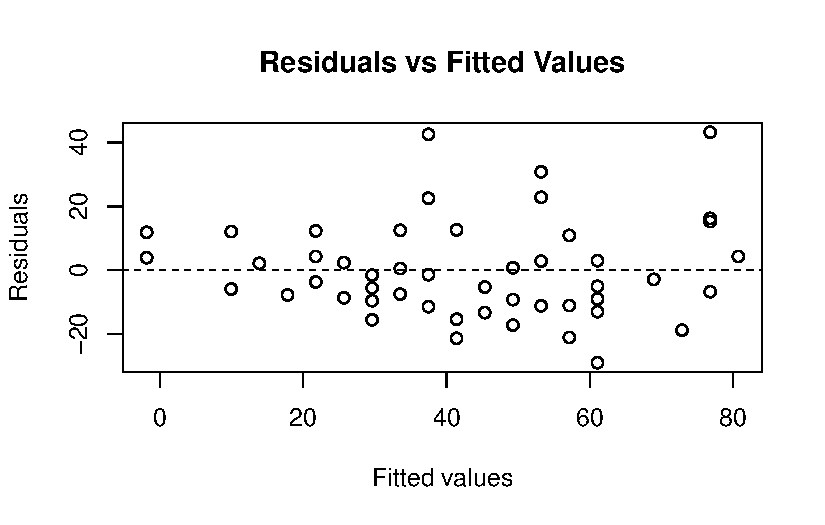
\includegraphics{HW8_files/figure-pdf/unnamed-chunk-7-1.pdf}

}

\end{figure}

\begin{Shaded}
\begin{Highlighting}[]
\CommentTok{\# F{-}test for equal variance}
\NormalTok{fitted\_vals }\OtherTok{\textless{}{-}} \FunctionTok{fitted}\NormalTok{(model\_cars)}
\NormalTok{high\_group }\OtherTok{\textless{}{-}} \FunctionTok{residuals}\NormalTok{(model\_cars)[fitted\_vals }\SpecialCharTok{\textgreater{}} \DecValTok{30}\NormalTok{]}
\NormalTok{low\_group }\OtherTok{\textless{}{-}} \FunctionTok{residuals}\NormalTok{(model\_cars)[fitted\_vals }\SpecialCharTok{\textless{}=} \DecValTok{30}\NormalTok{]}
\FunctionTok{var.test}\NormalTok{(high\_group, low\_group)}
\end{Highlighting}
\end{Shaded}

\begin{verbatim}

    F test to compare two variances

data:  high_group and low_group
F = 4.1325, num df = 34, denom df = 14, p-value = 0.006658
alternative hypothesis: true ratio of variances is not equal to 1
95 percent confidence interval:
 1.527594 9.415644
sample estimates:
ratio of variances 
          4.132502 
\end{verbatim}

Based on the plot it appears that there is an unequal distribution of
residuals in the plot which could suggest the zero mean error assumption
is violated.The F-test compares the variances of those with fitted
values greater than 30 (high\_group) and those with fitted values less
than or equal to 30 (low\_group). The p-value is less than 0.05,
indicating that there is a significant difference between the variances
of these groups. This suggests the presence of heteroscedasticity which
would violate the zero mean error assumption.

\hypertarget{b.-report-the-estimate-of-the-heteroscedastic-consistent-variance-for-the-regression-slope.}{%
\section{2.B. Report the estimate of the heteroscedastic consistent
variance for the regression
slope.}\label{b.-report-the-estimate-of-the-heteroscedastic-consistent-variance-for-the-regression-slope.}}

\begin{Shaded}
\begin{Highlighting}[]
\NormalTok{coef\_test }\OtherTok{\textless{}{-}} \FunctionTok{coeftest}\NormalTok{(model\_cars, }\AttributeTok{vcov =} \FunctionTok{vcovHC}\NormalTok{(model\_cars, }\AttributeTok{type =} \StringTok{"HC0"}\NormalTok{))}
\NormalTok{coef\_test}
\end{Highlighting}
\end{Shaded}

\begin{verbatim}

t test of coefficients:

             Estimate Std. Error t value  Pr(>|t|)    
(Intercept) -17.57909    5.54187 -3.1720  0.002639 ** 
speed         3.93241    0.39868  9.8636 3.964e-13 ***
---
Signif. codes:  0 '***' 0.001 '**' 0.01 '*' 0.05 '.' 0.1 ' ' 1
\end{verbatim}

\begin{Shaded}
\begin{Highlighting}[]
\NormalTok{hetvar }\OtherTok{\textless{}{-}}\NormalTok{model\_cars }\SpecialCharTok{\%\textgreater{}\%} 
  \FunctionTok{vcovHC}\NormalTok{() }\SpecialCharTok{\%\textgreater{}\%} \CommentTok{\# calculate Heteroscedasticity{-}consistent estimation of the covariance matrix for coefficients}
  \FunctionTok{diag}\NormalTok{() }\SpecialCharTok{\%\textgreater{}\%} \CommentTok{\# gives variances as they are the diagonal of the covariance matrix}
  \FunctionTok{sqrt}\NormalTok{() }\CommentTok{\# gives standard error as it is square root of variance}

\NormalTok{heteroscedastic\_variance }\OtherTok{\textless{}{-}}\NormalTok{ hetvar[}\DecValTok{2}\NormalTok{]}\SpecialCharTok{\^{}}\DecValTok{2}
\NormalTok{heteroscedastic\_variance}
\end{Highlighting}
\end{Shaded}

\begin{verbatim}
    speed 
0.1827881 
\end{verbatim}

\begin{Shaded}
\begin{Highlighting}[]
\FunctionTok{summary}\NormalTok{(model\_cars)}
\end{Highlighting}
\end{Shaded}

\begin{verbatim}

Call:
lm(formula = dist ~ speed, data = cars)

Residuals:
    Min      1Q  Median      3Q     Max 
-29.069  -9.525  -2.272   9.215  43.201 

Coefficients:
            Estimate Std. Error t value Pr(>|t|)    
(Intercept) -17.5791     6.7584  -2.601   0.0123 *  
speed         3.9324     0.4155   9.464 1.49e-12 ***
---
Signif. codes:  0 '***' 0.001 '**' 0.01 '*' 0.05 '.' 0.1 ' ' 1

Residual standard error: 15.38 on 48 degrees of freedom
Multiple R-squared:  0.6511,    Adjusted R-squared:  0.6438 
F-statistic: 89.57 on 1 and 48 DF,  p-value: 1.49e-12
\end{verbatim}

The estimate of the heteroscedastic consistent variance for the
regression slope is 0.1827881.

\hypertarget{c.-construct-95-confidence-interval-of-the-regression-slope-assuming-homoscedasticity-and-using-the-results-in-2.b.-how-do-they-compare}{%
\section{2.C. Construct 95\% confidence interval of the regression slope
assuming homoscedasticity and using the results in 2.B. How do they
compare?}\label{c.-construct-95-confidence-interval-of-the-regression-slope-assuming-homoscedasticity-and-using-the-results-in-2.b.-how-do-they-compare}}

\begin{Shaded}
\begin{Highlighting}[]
\CommentTok{\# Regular CI}
\FunctionTok{confint}\NormalTok{(model\_cars)}
\end{Highlighting}
\end{Shaded}

\begin{verbatim}
                 2.5 %    97.5 %
(Intercept) -31.167850 -3.990340
speed         3.096964  4.767853
\end{verbatim}

\begin{Shaded}
\begin{Highlighting}[]
\CommentTok{\# Robust CI}
\NormalTok{robust\_se }\OtherTok{\textless{}{-}} \FunctionTok{sqrt}\NormalTok{(}\FunctionTok{diag}\NormalTok{(}\FunctionTok{vcovHC}\NormalTok{(model\_cars, }\AttributeTok{type =} \StringTok{"HC0"}\NormalTok{)))}
\NormalTok{beta }\OtherTok{\textless{}{-}} \FunctionTok{coef}\NormalTok{(model\_cars)}
\NormalTok{robust\_ci }\OtherTok{\textless{}{-}} \FunctionTok{data.frame}\NormalTok{(}
  \AttributeTok{lower =}\NormalTok{ beta }\SpecialCharTok{+} \FunctionTok{qt}\NormalTok{(}\FloatTok{0.025}\NormalTok{, }\AttributeTok{df =} \FunctionTok{nrow}\NormalTok{(cars)}\SpecialCharTok{{-}}\DecValTok{2}\NormalTok{) }\SpecialCharTok{*}\NormalTok{ robust\_se,}
  \AttributeTok{upper =}\NormalTok{ beta }\SpecialCharTok{+} \FunctionTok{qt}\NormalTok{(}\FloatTok{0.975}\NormalTok{, }\AttributeTok{df =} \FunctionTok{nrow}\NormalTok{(cars)}\SpecialCharTok{{-}}\DecValTok{2}\NormalTok{) }\SpecialCharTok{*}\NormalTok{ robust\_se}
\NormalTok{)}
\NormalTok{robust\_ci}
\end{Highlighting}
\end{Shaded}

\begin{verbatim}
                 lower     upper
(Intercept) -28.721776 -6.436414
speed         3.130807  4.734010
\end{verbatim}

Regular CI: (3.096964, 4.767853). Robust CI: (3.130807, 4.734010)

While both intervals are fairly similar, the robust CI is slightly
shifted as both the lower and upper bounds are higher. The robust CI is
also more narrow, indicating that adjusting for heteroscedasticity
reduces the uncertainty around the estimate.

\hypertarget{d.-check-for-the-lack-of-fit-of-the-model.}{%
\section{2.D. Check for the lack of fit of the
model.}\label{d.-check-for-the-lack-of-fit-of-the-model.}}

\begin{Shaded}
\begin{Highlighting}[]
\CommentTok{\# Creating groups based on unique speed values}
\NormalTok{pure\_error\_model }\OtherTok{\textless{}{-}} \FunctionTok{lm}\NormalTok{(dist }\SpecialCharTok{\textasciitilde{}} \FunctionTok{factor}\NormalTok{(speed), }\AttributeTok{data =}\NormalTok{ cars)}
\FunctionTok{anova}\NormalTok{(model\_cars, pure\_error\_model)}
\end{Highlighting}
\end{Shaded}

\begin{verbatim}
Analysis of Variance Table

Model 1: dist ~ speed
Model 2: dist ~ factor(speed)
  Res.Df     RSS Df Sum of Sq      F Pr(>F)
1     48 11353.5                           
2     31  6764.8 17    4588.7 1.2369 0.2948
\end{verbatim}

The p-value is 0.2948 which indicates that pure\_error\_mode is not
significantly better than model\_cars. There is no lack of fit in
model\_cars, or the linear model.



\end{document}
